\documentclass{article}
\usepackage[utf8]{inputenc}
\usepackage{fullpage}
\usepackage{amsmath}
\usepackage{verbatim}
\usepackage{graphicx}
\usepackage{hyperref}
\hypersetup{colorlinks=true,linktoc=all}
\usepackage{listing}
\usepackage{subcaption}
\usepackage[table]{xcolor}
\usepackage{multirow}
\usepackage{cleveref}
\usepackage{xspace}

\newcommand{\filter}{\textit{Filter}\xspace}
\newcommand{\projection}{\textit{Projection}\xspace}
\newcommand{\join}{\textit{Join}\xspace}
\newcommand{\sort}{\textit{Sort}\xspace}
\newcommand{\indexing}{\textit{Indexing}\xspace}
\newcommand{\groupby}{\textit{Group By}\xspace}
\newcommand{\topk}{\textit{TopK}\xspace}


\title{In-Storage SQL Processing\\
  \large MIT CSAIL Joint Research Proposal} \author{Shuotao Xu, Xiangyao Yu\\
  CSG Group, DB Group\\
  (shuotao@csail.mit.edu), (yxy@csail.mit.edu)}

\begin{document}
\maketitle
\section{Introduction}
With the ever-growing data collected and available, technology for fast and efficient data storage is becoming increasingly crucial for supporting complex queries on large datasets.
For big-data applications, a large number of analytic platforms rely on relational database systems, such as MySQL and Postgres, to store large datasets and running complex SQL queries.
An SQL database system brings data from the flash disks via the interconnecting storage network to the CPU cache to perform analysis of the fetched data.

With today's technology advancement, the storage network I/O bandwidth can be imbalanced with the aggregate secondary storage bandwidth, and become a bottleneck for fast SQL processing.
Such a scenario can be true for both a single server and a cluster of servers for SQL processing.
On a single server node, a flash disk is typically connected via 4 lanes of PCIe gen3 bus, which provide 4GB/s of bandwidth.
The flash chips inside a flash disk can provide a internal aggregate bandwidth which is much greater than the PCIe gen3 bus, if they are organized in a parallel architecture.
Therefore, SQL processing on a single node can be bottlenecked by the PCIe bus bandwidth.
On the other hand, on the cluster of servers performing distributed SQL analysis, compute and storage components are typically separated on different physical servers, such as the Amazon cloud.
With such a compute and storage separation in a cloud, the distributed SQL processing performance can be also held up by the slow server network speed.

In today's flash storage technology development, industry as well as academia are trying to enable some in-storage computational capabilities, such as ARM processors and FPGAs, to application developers.
In this research, we want to investigate how to use such in-storage computation hardware to offload some of the SQL operators inside flash drives to boost SQL query performance.
We propose to investigate 7 important SQL operators for the benefits of in-storage processing: \filter, \projection, \join, \sort, \indexing, \groupby, and \topk.
We will devise new techniques to implement those operators on inside storage due to limited computation and DRAM size.
We assume that the IO-intensive operators such as \filter, \projection, \join, \sort, \groupby and \topk  will benefit the most from in-storage processing.
Operators, such as \sort, are compute-bound, which we assume will not benefit from in-storage computing.

Specifically, the proposed research will make the following contributions.

\begin{itemize}
\item We extensively study the widely used operators in SQL-based relational databases. For each operator, we conduct a qualitative analysis of whether it can benefit from near-storage computing. 

\item We design and optimize these operators in a near-storage computing platform and demonstrate a significant reduction in IO traffic and CPU computation time. 

\item We incorporate the design into an open-source database, SQLite, and evaluate the performance advantage of each optimization we propose. 
\end{itemize}

Please note that this MIT internal collaboration between Computer Structure Group and Database Group has been started prior to the Samsung Internship. And we are interested in pursuing this research in an open-source domain.


\section{System Architecture}

A relational query processor takes a declarative SQL statement, validates it, optimizes it into a procedural dataflow execution plan, and execute that dataflow program on behalf of a client.
A relational query processor typically have four major software components 1) Query Parser, 2) Query Rewriter, 3) Query Optimizer and 4) Plan Executor.
The first three components generate a query plan, and the Plan Executor then issues disk IOs to the storage device, and execute the plan as shown in Figure~\ref{fig:software}.
In this proposal, we want to modify the Plan Executor such that it adds a side channel to the storage device.
Via this side channel, IO-intensive operations can be offloaded to the accelerators in the flash drive, as shown in Figure~\ref{fig:accelerator}.
As a result of such a in-storage accelerator architecture, 1) the total IOs between the processor and storage are dramatically reduced, and 2) accelerators can utilize the entire aggregate internal NAND flash bandwidth.

\begin{figure}[!htb]
  \centering
    \begin{subfigure}[t]{0.40\textwidth}
      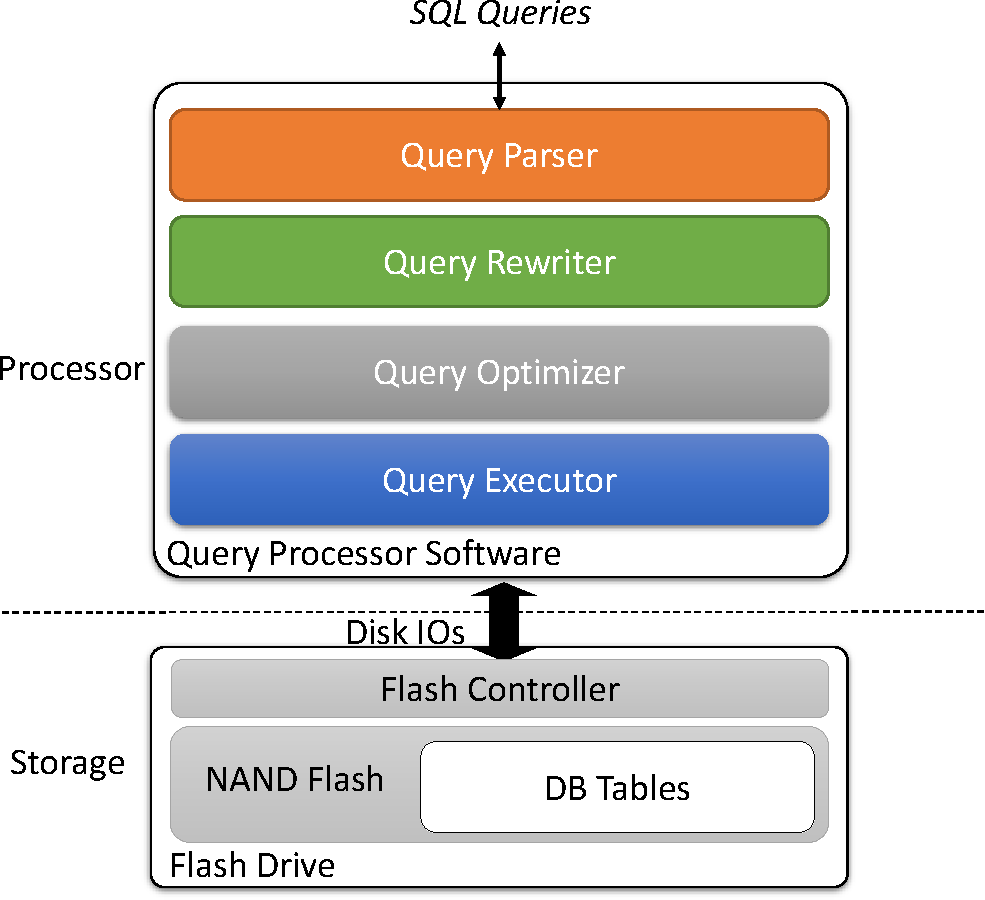
\includegraphics[width=\textwidth]{figures/software-stack-crop.pdf}
      \caption{Traditional Query processing stack}
      \label{fig:software}
  \end{subfigure}\hspace{5pt}
  \begin{subfigure}[t]{0.40\textwidth}
    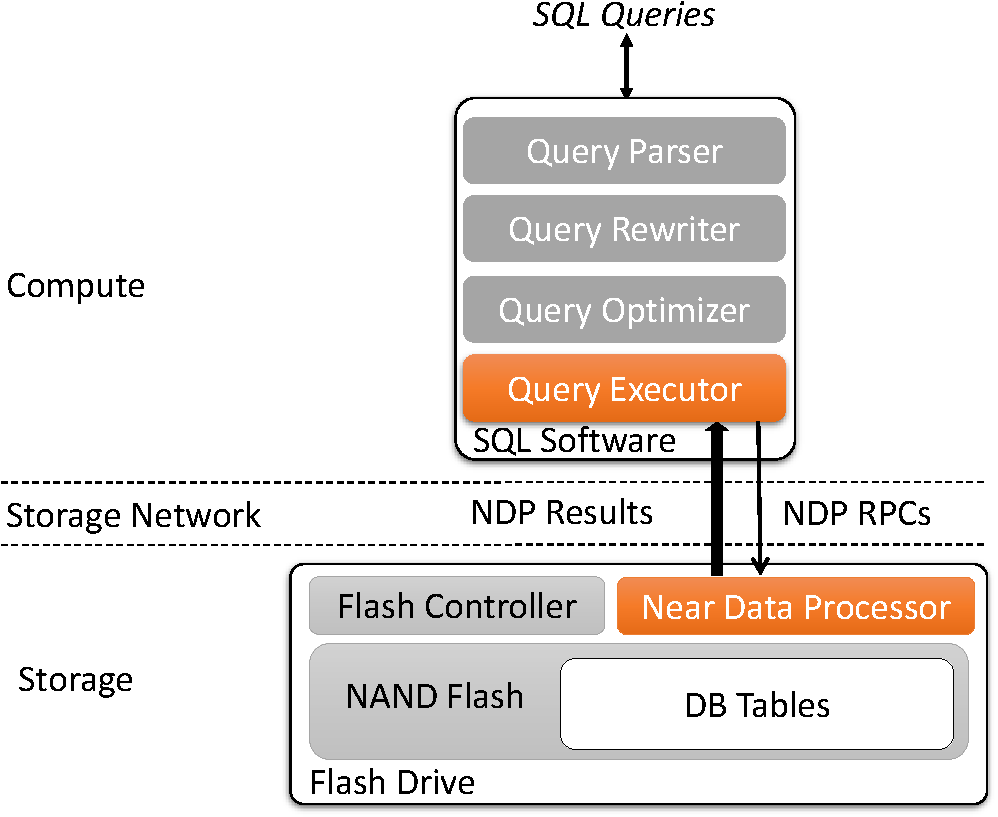
\includegraphics[width=\textwidth]{figures/accelerator-stack-crop.pdf}
    \caption{Query processing stack with In-storage Accelerators}
    \label{fig:accelerator}
  \end{subfigure}
  \label{fig:try}
  \caption{DBMS Query Processing Architectures}
\end{figure}

\section{SQL Operators}

In this section, we investigate seven most commonly used operators in a database qualitatively and discusses whether they are amenable to near-data computing (\cref{sec:analysis}). Then, we discuss how each individual operators can be performed using NDP from Section~\ref{sec:xxx} to \ref{sec:xxx}.

\subsection{Qualitative Analysis of Operators} \label{sec:analysis}

Table~\ref{tab:operators} presents the seven operators that we focus on. For each operator, we present the average time complexity for a typical implementation, the worse case space complexity, and whether the operator is amenable to NDP.
If the operator is on a single table, $N$ represents the size of that table; if the operator is on two tables, $N$ ($M$) represents the size of the smaller (bigger) table. 
For the \textit{Group By} operator, $K$ is the number of groups. For the \textit{TopK} operator, $K$ is the number of records selected. 

\begin{table}
\centering 
\begin{tabular}{ |c|c|c|c| } 
 \hline
 Operator       & Time Complexity & Space Complexity  & Amenable to NDP \\ \hline
 \filter        & $\Theta(N)$     & $\Theta(1)$       & Yes             \\ \hline
 \projection    & $\Theta(N)$     & $\Theta(1)$       & Yes             \\ \hline
 \indexing      & $\Theta(\log{N})$ & $\Theta(N)$     & Yes             \\ \hline
 \join          & $\Theta(M + N)$ & $\Theta(N)$       & Yes (Partial)   \\ \hline
 \groupby       & $\Theta(N)$     & $\Theta(K)$       & Yes (Partial)   \\ \hline
 \topk          & $\Theta(N\log{K})$ & $\Theta(K)$    & Yes (Partial)   \\ \hline
 \sort          & $\Theta(N\log{N})$ & $\Theta(\log{N})$ & No           \\ \hline
\end{tabular}
\caption{Comparison of common SQL operators.}
\label{tab:operators}
\end{table}

Among the seven operators, some are very amenable to NDP (i.e., \filter and \projection) as they can be performed at wire speed as the data is loaded from the storage device. It is more difficult to implement some other operators (i.e., \join, \groupby, \indexing, \topk) using NDP as they require considerable computation and intermediate states which the current-generation near-storage processors do not readily support. We will investigate how these operators can be broken down into smaller operators that are more amenable to NDP. 
Finally, the operator \sort is not amenable to NDP as it requires too much computation and storage such that it is more appropriate to execute it at the host. 

For the rest of this section, we will discuss our proposed implementation for \filter, \projection, \join, \groupby, \indexing, and \topk.


\subsection{Join}

An SQL JOIN operation combines columns from one or more tables in a relational database.
A popular implementation of JOIN operations uses the hash join algorithm.
JOIN is typically IO-intensive operations because all rows of the joining tables have to be read from the secondary storage.

As show in Figure~\ref{fig:hash-join}, to hash-join Table A and B, a hash table is first constructed with values of the departmentID column in table A.
Then the values of the departmentID column in table B are fetched to find a match in the hash table.
Such an algorithm requires all the data records to be retrieved from the secondary storage to CPU.

We propose accelerator for hash-join which implements a in-storage bloom-filter in datapath as shown in Figure~\ref{fig:filter-hash-join}.
When rows of table A is read from flash to CPU for the hash table construction, it constructs a bloom-filter in the datapath.
When the rows of table B are streamed from flash to join the hash table, they are filtered with the constructed bloom filter before sending to CPU.
If the bloom-filter selectivity is high, i.e., only a relatively few rows need to be joined, such a mechanism can greatly reduced required IO from storage to CPU.

\begin{figure}[!htb]
  \centering
  \begin{subfigure}[t]{0.48\textwidth}
    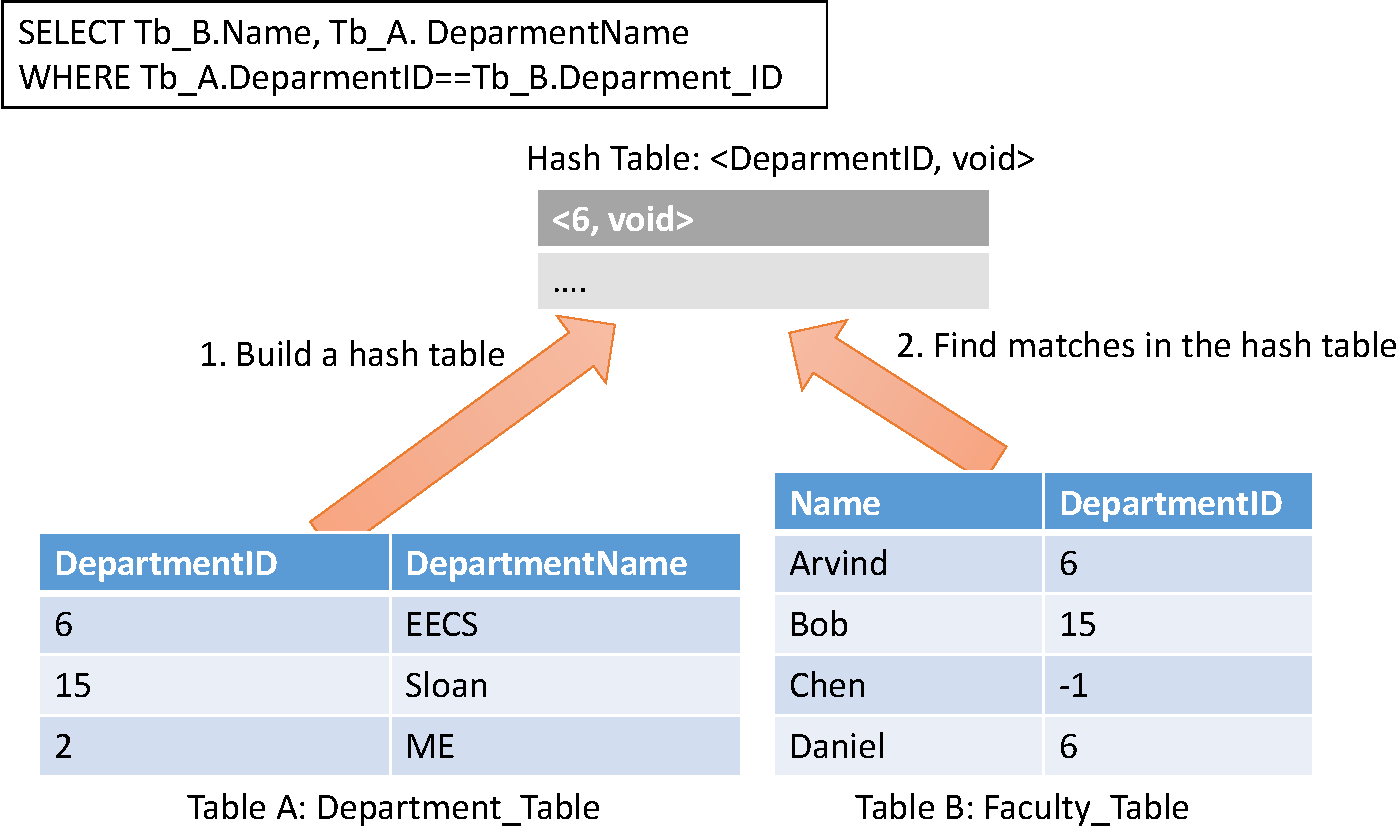
\includegraphics[width=\textwidth]{figures/hash-join-crop.pdf}
      \caption{Hash-join Operations without accelerators}
      \label{fig:hash-join}
  \end{subfigure}
  \begin{subfigure}[t]{0.48\textwidth}
    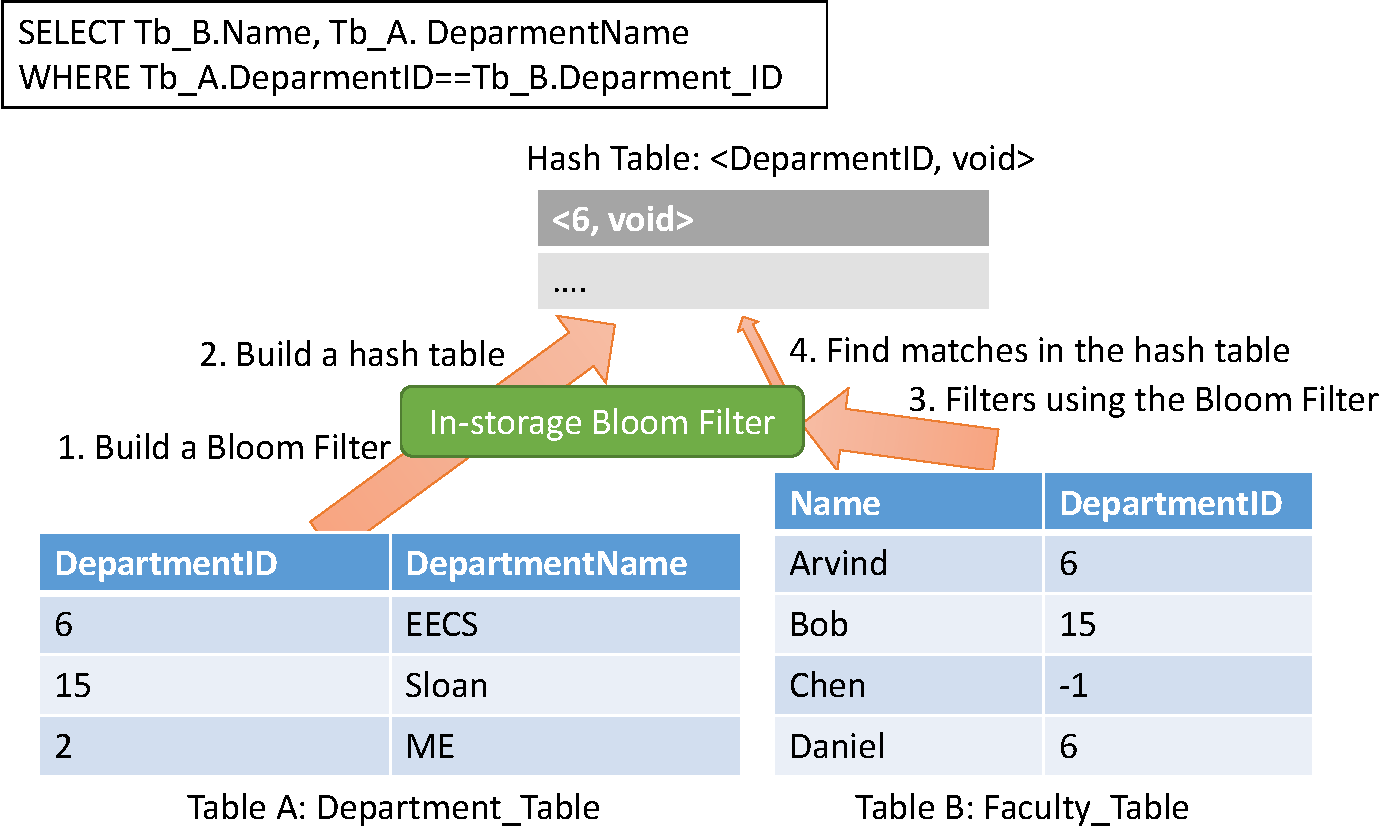
\includegraphics[width=\textwidth]{figures/filter-hash-join-crop.pdf}
    \caption{Accelerated Hash-join Operations with In-storage Bloom filter}
    \label{fig:filter-hash-join}
  \end{subfigure}
  \label{fig:try}
  \caption{Hash-join Operations}
\end{figure}

\subsection{TopK}

\topk selects the top K-th attributes from the table.
One can dramatically reduce the IO from SSD from CPU by processing \topk operator in storage.
By offloading \topk operator to SSD, one can reduce the disk IO by k/N, where N the total number of rows of a table.
We can implement an FPGA-based parallel sorting network for 2K tuples, and throw away the bottle K tuples.
Such fast sorting network has been explored by work such as ~\cite{fpga-sort}.

\subsection{Index Probing}
\indexing are used in SQL queries to pinpoint row data locations when a certain column has a index.
Probing a b-tree index typically requires $\log{N}$ reads from SSDs, and the read latencies are additive.
If we offload  the index probing on in-storage processors, the latencys of \indexing operations can be greatly improved, because the slow storage network access is avoided.

\subsection{Filter and Projection}

A filter operator will filter out database rows based on the predicate.
Likewise a projection operator will take the selected columns from database rows.
The computation of the filter and projection operators only needs one pass of the data and has little DRAM requirement.
Thus, it is straightforward to implement on in-storage processing unit.
Such a work has been extensively explored by work such as IBM Nettezza~\cite{netezza}.

\subsection{Group-By Aggregate}

Aggregate functions are often used with \groupby database operations, where rows are grouped based on column values and each group of rows is summarized by applying the aggregate functions.
When number of groups are much smaller than total number of rows in a table, storage IO can be greatly reduced by offloading aggregate functions with GROUPBY to the flash drive.
Previous work, Ibex~\cite{ibex} has investigated how aggregate group-by works on FPGA.


%% \subsection{Sort Accelerator}


\section{Evaluation Benchmarks}
\label{sec:eval}
To evaluate the work, we propose to run some synthetic SQL queries with aggregate functions and join, as well as some queries from TPC-H, and TPC-DS.
By comparing the same query on the same dataset running on the traditional relational database systems, such as MySQL and Postgres, we can illustrate the performance benefits of the new architecture with accelerators.

Below are examples of SQL queries we plan to evaluate.

\begin{enumerate}

\item Query A: Synthetic query for evaluating aggregate accelerator 
\begin{verbatim}
SELECT department, years in company, SUM(salary) as sal sum
FROM employee GROUP BY department, years_in_company
\end{verbatim}

\item Query B: Modified Q14 of TPC-H for evaluating hash-join accelerator
\begin{verbatim}
SELECT sum(l_extendedprice * (1-l_discount)) as promo_revenue
FROM lineitem, part
WHERE l_partkey = p_partkey
and l_shipdate >= 1995-09-01 
and l_shipdate < 1995-10-01
\end{verbatim}

\item Query C: Q52 of TPC-DS for evaluating complex queries by both accelerators
\begin{verbatim}
SELECT dt.d_year, item.i_brand_id brand_id, item.i_brand brand,
SUM(ss_ext_sales_price) ext_price
FROM date_dim dt, store sales, item
WHERE dt.d date sk = store sales.ss sold date sk AND
store sales.ss item sk = item.i item sk AND
item.i manager id = 1 AND dt.d moy = 11 AND dt.d year = 2000
GROUP BY dt.d year, item.i brand, item.i brand id
ORDER BY dt.d year, ext price DESC, brand id
\end{verbatim}
\end{enumerate}

\bibliographystyle{abbrv}
\bibliography{reference}

\end{document}



